%!TEX root = ../thesis-main.tex
\chapter{\conclusionsname}
\label{chap:conclusions}
The objective of this thesis was clear, but the solution to achieve was not immediately apparent. An agile project development methodology helped in gradually reaching a solution step by step. A long analysis phase was useful to identify potential solutions, but many of these solutions were found to have significant drawbacks that made them unsuitable.\newline

\centerImage{figures/swingui.png}{Dodgeball simulation in Alchemist Swing UI}{swingui}{1}

Kotlin Multiplatform was eventually identified as the best solution for this particular scenario. It is a relatively new technology with the potential to grow, allowing the Alchemist Web Render project to do the same. By creating an initial proof of concept, it was possible to demonstrate that the project's goal could be achieved by developing a solid and well-architected solution.\newline

An example dodgeball simulation is presented, extrapolated from an example in the
Alchemist tutorial~\cite{Coordination2021-alchemist-tutorial}, where some nodes pass a ball to each other randomly, and each node keeps count of how many times it receives the ball. The simulation involves a network of nodes that collaborate to utilize a shared set of resources. To prevent conflicts, neighboring nodes generate and trade resource usage tokens, ensuring that each resource is only used by a single node at any given time. A sample frame of this simulation can be displayed in the classic swing UI, as shown in \fullref{fig:swingui}.\newline

\centerImage{figures/web-renderer.png}{Dodgeball simulation in Alchemist Web Renderer}{web-renderer}{0.6}

Using the Alchemist Web Renderer, the same simulation can be monitored, an example of a frame is depicted in \fullref{fig:web-renderer}.The resulting image in this second case would have been exactly the same, independently by the fact that it was rendered using the Computation on Server approach or the Computation on Client approach. The ``effect" used to personalize the colors of the nodes in this visualization is not the same used in the swing UI, but it has been created using almost the same principles so that it was possible to visualize a similar image. The node color is black if it currently has got the ball in both the images. The nodes slowly shift towards other colors depending on how many time they received a ball.\newline

At present, the project remains in its nascent stage, and a considerable number of features need to be incorporated. Some of these potential features are described in \fullref{sec:future-works}. The principal aim of this thesis was to establish a solid foundation that would facilitate the seamless addition of features in the future, while minimizing modifications in the existing architecture.\newline

At the current stage of development, profiling performance may not be a highly useful exercise, as there are numerous aspects of the project that can be improved. It is worth noting that the primary objective of this research was not to achieve optimal performance, which remains a significant challenge in this particular scenario. Therefore, the focus has been primarily on establishing a solid foundation that can facilitate the development of new features with relative ease, while addressing the known performance issues as development progresses.\newline

Along with some considerations, some data is still being presented. The measurements were performed on a single machine, where both the Server and the Client components are located. The machine has limited hardware capabilities, and is characterized by the following specifications:

\begin{itemize}
	\item \textbf{Processor}: Intel(R) Core(TM) i5-2520M CPU @ 2.50GHz
	\item \textbf{RAM}: 8GiB System memory
	\item \textbf{GPU}: 2nd Generation Core Processor Family Integrated Graphics Controller
\end{itemize}

\paragraph{Free variables}
The two free variable in the measurements are:
\begin{enumerate}
	\item the number of nodes $N$ ($N \in \mathbb{N}^{+}$) participating in the system, representing the size of the monitored system;
	\item The utilized approach (Computation on Server or Computation on Server).
\end{enumerate}
\paragraph{Metrics}
The four metrics measured to evaluate the performance of the system are:
\begin{enumerate}
	\item \textbf{rendering time}: the time required by the renderer component to complete its execution, this
	metric is meant to compare the raw performance of the renderer across the available platforms. The execution on the JVM is expected to be faster than the one on the browser;
	\item \textbf{serialization time}: the time required by the Server to serialize the \textit{Environment State} (in the Computation on Client approach) or the rendered image (in the Computation on Server approach). This operation is always accomplished by the Server;
	\item \textbf{deserialization time}: the time required by the Client to deserialize the \textit{Environment State} (in the Computation on Client approach) or the rendered image (in the Computation on Server approach). This operation is always accomplished by the Client;
	\item \textbf{total time}: the time required to complete an entire iteration, which includes all the previous metrics plus the network delay.
\end{enumerate}

Each metric is measured five times, and the presented results are an average of such data.

\paragraph{Final Results}
The results are presented and summarized in \fullref{fig:performace-graphs}. As anticipated, utilizing the Computation on Server approach yields more stable system performance as the monitored system expands. This is mainly due to the JVM's superior efficiency in comparison to Javascript. Additionally, the JVM is consistently faster in rendering the system and surprisingly quicker in converting the model into an image format than in plain JSON. Nevertheless, this is highly reliant on the specific serialization formats and libraries employed, and may drastically change with different implementations. Finally, it is apparent that adopting the Computation on Client approach is quite effective for minor systems, but it becomes less scalable than the Computation on Server strategy as the environment size expands.
\begin{center}
	\begin{figure}[htb]
		\centering
		\begin{subfigure}[t]{0.45\textwidth}
			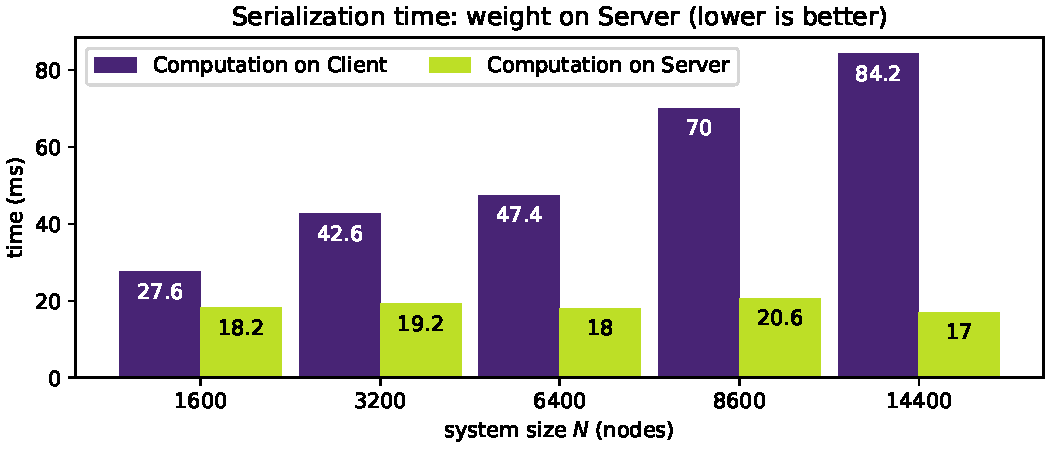
\includegraphics[width=0.99\textwidth]{figures/serialization-time}
		\end{subfigure}%
		~
		\begin{subfigure}[t]{0.45\textwidth}
			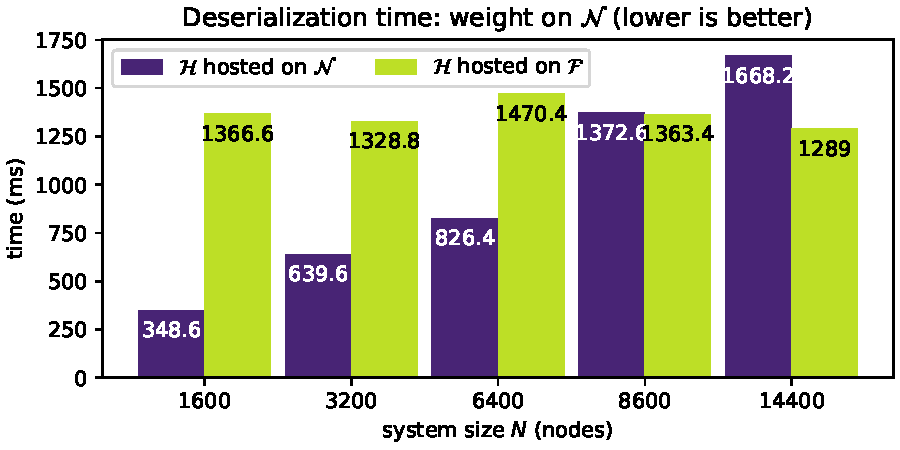
\includegraphics[width=0.99\textwidth]{figures/deserialization-time}
		\end{subfigure}
		~
		\begin{subfigure}[t]{0.45\textwidth}
			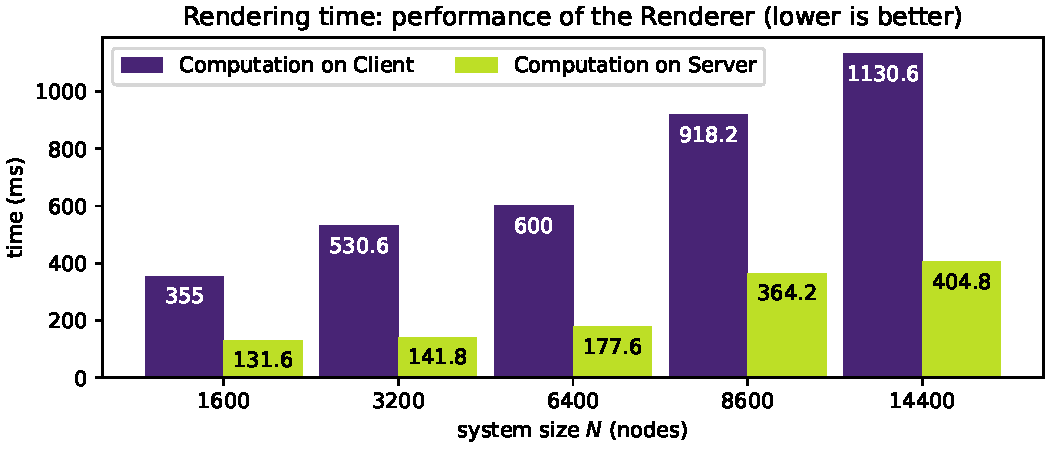
\includegraphics[width=0.99\textwidth]{figures/rendering-time}
		\end{subfigure}
		~
		\begin{subfigure}[t]{0.45\textwidth}
			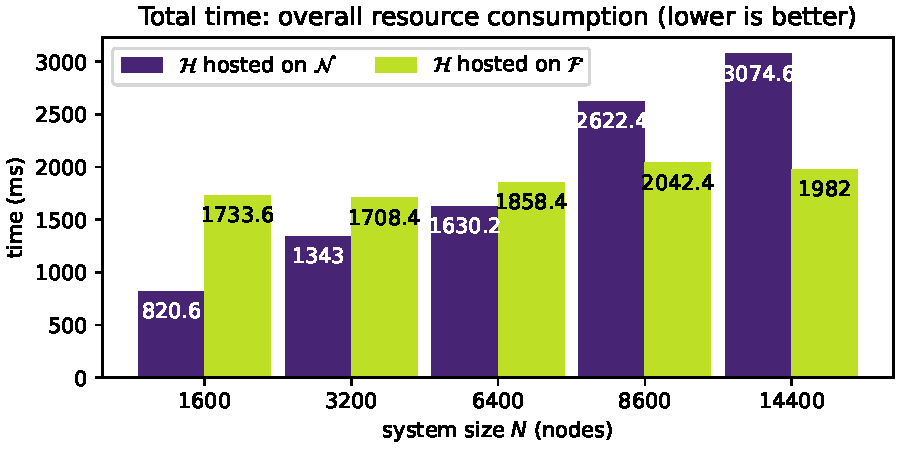
\includegraphics[width=0.99\textwidth]{figures/total-time}
		\end{subfigure}
		\caption{Performance evaluation}
		\label{fig:performace-graphs}
	\end{figure}
\end{center}

In conclusion, this project thesis has successfully fulfilled its objective of creating a foundation for the future works of the Alchemist Web Renderer project, and provides a clear path forward for continued growth and progress.\newline

\section{Future Works}
\label{sec:future-works}
The objective of this project thesis was to prove the feasibility of developing a flexible and cross-platform renderer for the Alchemist Simulator and to lay the foundation for a solid and functional structure for future works. A robust architecture has been established that can serve as the foundation for future advancements in this field. With this foundation in place, it is now possible to progressively add new features and capabilities that can build upon and enhance the existing structure. The following features are among the most notable and yet to be implemented:
\begin{itemize}
	\item \textbf{Improvement in Performances}: An analysis on how to enhance the system's performance is necessary, considering the data presented in \fullref{chap:conclusions}. The performance of this type of system will always be crucial, and even if most of the issues related to serialization are resolved, it may not be sufficient. However, there are several strategies that could be implemented to circumvent this problem:
	\begin{itemize}
		\item \textbf{Best Effort Strategy}: by using this strategy, only the most recent information is displayed while the simulation continues to run, resulting in the loss of some events. Although this approach is already implemented, it could also be rethought using WebSockets. This strategy is efficient in terms of time, but is not ideal for simulations where the precision factor is crucial;
		\item \textbf{Wait Strategy}: the Simulation Engine halts until the current state of the environment is rendered and displayed to the user. This technique necessitates the use of WebSockets, which will be elaborated later on in this list.
	\end{itemize}
	\item \textbf{Batch Mode Support}: Alchemist provides the ability to run multiple simulations using a single configuration that specifies multiple parameters. However, batch mode is not yet supported by the Alchemist Web Renderer project. To implement this feature, both the structure of the Server state and the client-side GUI needs to be updated. The API endpoints behaviors will require modification as well.
	\item \textbf{Websockets for Pull and Push operations}: Currently, the system operates on a REST architecture, where clients send requests to the server, which responds with the requested information. The server never actively sends data to clients. To change the interaction approach, the system could be updated to use a pull-push Websocket architecture, which would allow the server to push data to clients when needed (for example everytime the environment gets updated). This approach would require some changes to the way the client and server interact, but the underlying logic of the system should not change drastically.
	\item \textbf{Incarnations Support}: Each Incarnation in the project represents a distinct world with a unique concentration type and structure. Currently, the nodes of environments only supports position and do not contains information about the concentration. To support a particular Incarnation, it is necessary to create specific surrogate classes starting from the original concentration classes of that Incarnation. Mapping functions from the original class to the surrogate one should also be created. Once these steps have been completed, the polymorphic serializer will automatically handle the serialization and deserialization process for the supported Incarnations.
	\item \textbf{SVG based Renderer}: The SVG format offers several significant advantages over raster images. In order to take advantage of these benefits, a library that specializes in vector image creation must be adopted to create a Render implementation.
	\item \textbf{Body Compression Optimization}: Ktor offers the ability to compress the body of HTTP messages using the gzip algorithm. The aim is to significantly reduce the size of the payload being sent over the network, resulting in faster transfer speeds and lower bandwidth usage. While gzip is an effective algorithm, it may not always be the most efficient choice, especially for real-time compression scenarios. To address this issue, Ktor provides the flexibility to create custom components that deal with compression\footnote{https://ktor.io/docs/compression.html}. A possible algorithm that could be used in this case is the Zstandard\footnote{https://facebook.github.io/zstd/} from Facebook, which is a fast lossless compression algorithm that is specifically designed for real-time compression scenarios. In order to accomplish this objective, it is necessary to design and develop specific components that can be integrated into the Ktor project specific configuration.
	\item \textbf{Other Serialization Format Support}: The current implementation of the Alchemist Web Renderer project is limited to utilizing the JSON format for serialization. While this choice was made for valid reasons, exploring other serialization formats or adapting the format based on the project's development or production stage could offer benefits. The \textit{kotlinx.serialization} library offers a wide range of formats, and the ktor library integrates smoothly with it, making it simple to switch between formats. To achieve this objective, the necessary dependencies must be added to the build, and the polymorphic serialization issue discussed in \fullref{ssec:polymorphic-serialization} must be addressed. Once the Server is properly configured for content negotiation, ktor will be able to seamlessly handle different serialization formats.
	\item \textbf{Use platform specific libraries for Renderer component development}: In ~\fullref{ssec:renderer} it was discussed how the Renderer component can not use any platform-specific library. Many popular rendering and animation libraries are developed for JavaScript. However, the possibility to run JavaScript on a JVM was never pointed out as an option. It would be necessary to conduct a study to ascertain whether a satisfactory outcome can be obtained.
\end{itemize}
